\section{Introduction to Doxygen}
\begin{figure}[!ht]
\centering

\includegraphics[width=0.5\textwidth]{images/doxygen_logo.png}                   
\caption{Doxygen Logo}
\hspace{-1.5em}
\end{figure}
\noindent Doxygen is a documentation generator, a tool for writing software reference 
documentation. The documentation is written within code, and is thus 
relatively easy to keep up to date. Doxygen can cross reference 
documentation and code, so that the reader of a document can easily 
refer to the actual code.

Doxygen is the standard tool for generating documentation from
annotated C++ sources, but it also supports other popular programming
languages such as C, Objective-C, C\#, PHP, Java, Python, IDL (Corba
and Microsoft flavors), Fortran, VHDL, Tcl, and to some extent D.

\subsection{Features of Doxygen}
\begin{itemize}
\item Requires very little overhead from the writer of the documentation. 
Plain text will do, Markdown is support, and for more fancy or structured 
output HTML tags and/or some of doxygen's special commands can be used.
\item Cross platform: Works on Windows and many Unix flavors (including 
Linux and Mac OS X).
\item Comes with a GUI frontend (Doxywizard) to ease editing the options 
and run doxygen. The GUI is available on Windows, Linux, and Mac OS X.
\item Automatically generates class and collaboration diagrams in HTML 
(as clickable image maps) and $\mbox{\LaTeX}$ (as Encapsulated PostScript 
images).
\item Allows grouping of entities in modules and creating a hierarchy 
of modules.
\item Doxygen can generate a layout which you can use and edit to change 
the layout of each page.
\item Can cope with large projects easily.
\end{itemize}

\subsection{Installation of Doxygen}
Run following command in terminal:
\begin{verbatim}
$ sudo apt-get install doxygen
\end{verbatim}

\subsubsection{Usage}
It’s very simple to use. Just type \$ doxygen in terminal and you got
its manual.\\
To create documentation, move to folder where your source file exits
through terminal and then type
\begin{verbatim}
$ cd /path/to/your/project/source/
$ doxygen -g [filename]
\end{verbatim}

You can fill any filename as your choice. Its configuration file and
you can edit that according your project details like change project
name in filename.(config file for doxygen)

Then run

\begin{verbatim}
$ doxygen [filename]
\end{verbatim}

By this your documentation will be generated. This will create 2
folders in your current directory.

Folders: 

\begin{itemize}
\item {\bf html} for html documentation open
/path/to/project/source/html/index.html to check documentation.
\item {\bf latex} latex for documentation using latex as pdf output.
For that file run
\begin{verbatim}
$ cd /path/to/your/project/source/latex
$ make
\end{verbatim}
\end{itemize}

This will create refman.pdf file(check pdf file as file name may be
changed in your case).
\begin{figure}[!ht]
\centering
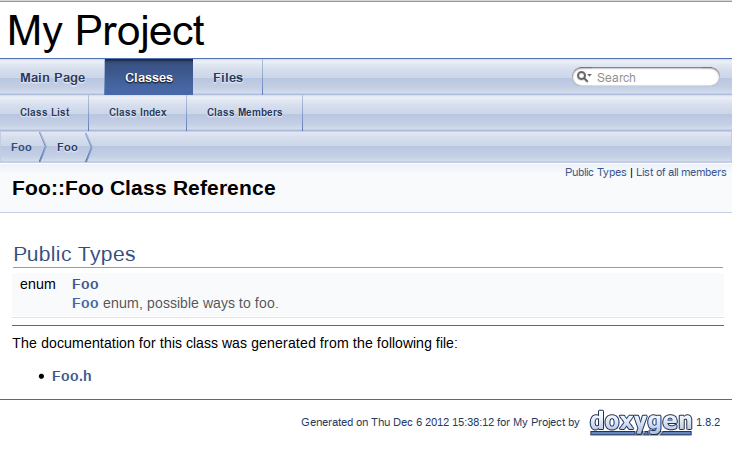
\includegraphics[width=0.7\textwidth]{images/doxygen_html.png}                   
\caption{Documentation using Doxygen}
\hspace{-1.5em}
\end{figure}
